\begin{figure*}[t]
\centering
\begin{subfigure}{0.37\textwidth}
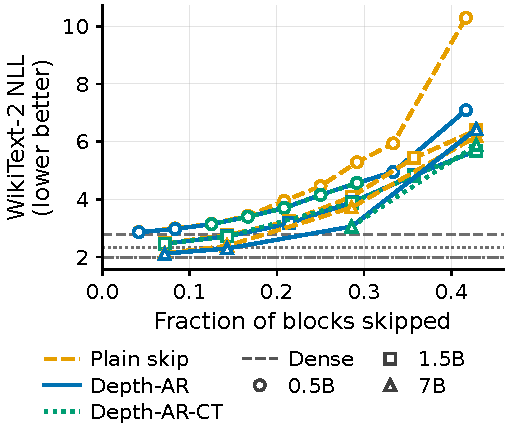
\includegraphics[width=\linewidth]{figures/fig2a_frontier.pdf}
\caption{The quality--compression frontier.}
\label{fig:frontier}
\end{subfigure}
\hfill
\begin{subfigure}{0.37\textwidth}
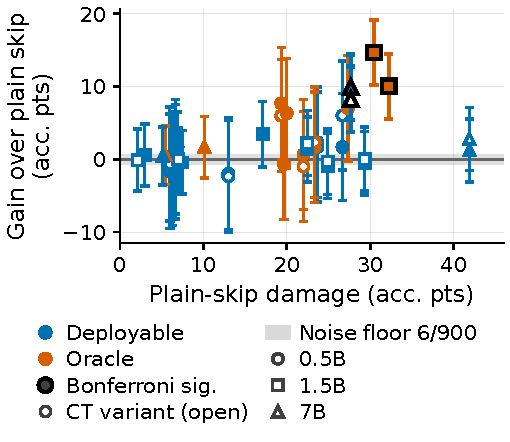
\includegraphics[width=\linewidth]{figures/fig2b_significant_gains.pdf}
\caption{Gain against damage.}
\label{fig:gains}
\end{subfigure}
\caption{\textbf{Significant gains appear only where skipping does severe damage.}
\emph{Left:} WikiText-2 NLL against the fraction of blocks skipped, for Qwen2.5-0.5B (circles),
1.5B (squares) and 7B (triangles), layers chosen by measured residual damage, every predictor
skipping identical blocks. \mname sits below plain skipping at every measured fraction on 0.5B
and 1.5B; dashed lines are the dense models. \emph{Right:} every accuracy comparison in the
paper, plotted as gain over plain skipping against the damage plain skipping does. Bars are
$95\%$ confidence intervals; the grey band is the evaluation's own measured reproducibility
floor, replicated after the main analysis closed (6 answers of 900, or $0.67$ accuracy points,
in BF16; \Cref{sec:app-noise}). Gains sit on zero where damage is small. Every comparison
surviving Bonferroni correction across all 63 tests (filled) lies at the right, at damage above
$27.7$ points, under both the deployable and the recovery-maximising rule. Severe damage is
necessary for a significant gain, and not sufficient: several badly damaged cells show none.
Hardware and protocol: \Cref{sec:app-protocol}.}
\label{fig:gains-pair}
\end{figure*}
